\section{Experiment: Bipedal Walker}

\subsection{Experimental Setup}

\subsubsection{Environment: OpenAI Gym – BipedalWalker-v3}
The BipedalWalker-v3 environment (shown in fig. \ref{fig:bwe}) from OpenAI Gym \cite{openai2021bipedalwalker} was selected as the benchmark for evaluating the performance of the continuous control algorithms. This environment represents a complex continuous control task, where a bipedal robot must learn to walk efficiently without falling.\\

\begin{figure} % Use figure* for full-width in twocolumn
    \centering
    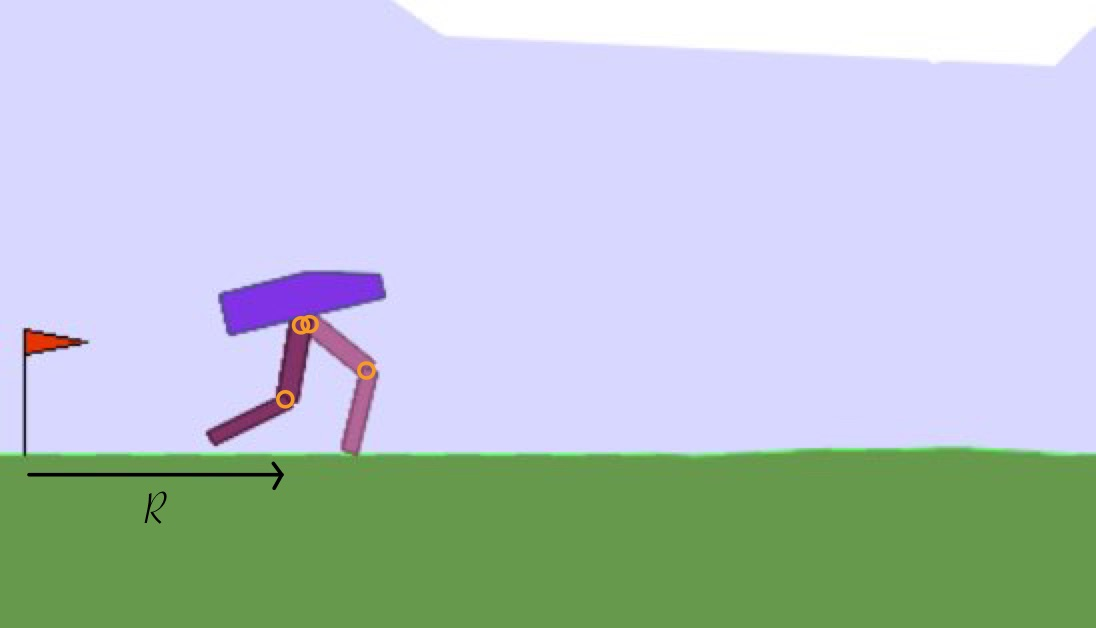
\includegraphics[width=0.45\textwidth]{BipdalWalker-1.jpg} % Passe den Dateinamen und Pfad an
    \caption{Bipedal Walker Environment}
    \label{fig:bwe}
\end{figure}

\noindent The simulation provides an approximation of bipedal locomotion dynamics and includes the following components \cite{pylessons2021bipedalwalker}:

\begin{itemize}
    \item State Space: A 24-dimensional vector representing the robot’s positional and velocity data, joint angles, and foot-ground contact information.
    \item Action Space: A 4-dimensional continuous vector with values in the range [-1,1], representing the torque applied to the four joints (hip and knee for both legs).
    \item Reward Function: The reward is composed of multiple elements: \begin{itemize}
        \item Positive reward for forward movement.
        \item Penalty for energy consumption (high torque usage).
        \item Penalty for falls.
        % \item A terminal reward of +300 when reaching the goal
    \end{itemize}
    
\end{itemize}

\subsubsection{Specific Challenges}
The BipedalWalker environment poses several challenges that make it a demanding benchmark for continuous control algorithms.

\begin{itemize}
    \item Instability: Maintaining dynamic balance is a non-trivial control problem.
    \item Sparse Rewards: Delayed and infrequent reward signals complicate exploration.
    \item Long-Term Planning: The agent must plan multiple steps ahead to develop a stable walk.
    \item High Dimensionality: The combination of a large state and action space requires function approximation.
\end{itemize}

\subsubsection{Training Parameters}

\newacronym{SB3}{SB3}{Stable Baselines 3}

In the experiments we used the \gls{SB3} \cite{stablebaselines3docs2023} library, which provides standardized and efficient implementations of various continuous control algorithms. To ensure a fair comparison, all three algorithms (\gls{DDPG}, \gls{PPO}, and \gls{SAC}) were trained using identical or analogous hyperparameters. The exact hyperparameter configurations used in the implementation are available at our Github Repository \cite{kreil2025github}. The shared hyperparameters are:
\begin{itemize}
    \item Learning rate: $3 \times 10^{-4}$
    \item Discount factor ($\gamma$): $0.99$
    \item Policy: MlpPolicy
\end{itemize}

\noindent For each of the three algorithms, we conducted 5 separate training runs with identical hyperparameters but different random seeds to ensure reliability of results and enable statistical comparability.

\subsubsection{Network Architecture}

All algorithms use the default MlpPolicy from \gls{SB3}, resulting in comparable network structures.

\subsubsection{Evaluation Metrics}

The following metrics were used to compare performance:

\begin{itemize}
    \item Training efficiency: Number of environment interactions required to achieve stable performance.
    \item Stability: Variance in performance across different training runs.
    \item Training Time: The actual wall-clock time required to train the agent.
\end{itemize}

\subsection{Results and Analysis}

\subsubsection{Learning Curves}

\begin{figure}[h] % Use figure* for full-width in twocolumn
    \centering
    \includegraphics[width=0.45\textwidth]{Comparison_of_algorithms.png} % Passe den Dateinamen und Pfad an
    \caption{Learning curves for \gls{DDPG}, \gls{PPO}} and \gls{SAC}
    \label{fig:algo_comperison}
\end{figure}

\noindent The learning dynamics vary significantly across the three algorithms, with the shaded regions in Figure \ref{fig:algo_comperison} representing the standard deviation across all five runs with different random seeds:

\begin{itemize}
    \item \gls{DDPG} (blue): Displays the slowest convergence and only attains \textasciitilde0 reward points at its best, followed by performance decline, which indicates serious stability issues.
    \item \gls{PPO} (green): Converges more slowly, reaching \textasciitilde180 reward points after \textasciitilde400,000 timesteps, with greater fluctuations during training.
    \item \gls{SAC} (red): Converges the fastest and reaches a stable performance level of \textasciitilde280 reward points after \textasciitilde300,000 timesteps.
\end{itemize}

\begin{table}[h]
\scriptsize
\centering
\begin{tabular}{@{}p{1.4cm}p{2.5cm}p{1.2cm}p{2.4cm}@{}}
\toprule
\textbf{Algorithm} & \textbf{Convergence Speed} & \textbf{MaxReward}\\
\midrule
\gls{DDPG} & Low (>500k steps)                  & \textasciitilde0\\
\gls{PPO}  & Medium (\textasciitilde400k steps) & \textasciitilde200\\
\gls{SAC}  & High (\textasciitilde300k steps)   & \textasciitilde300\\

\bottomrule
\end{tabular}
\caption{Comparison of Convergence Speed and Stability}
\end{table}

\noindent \gls{SAC} achieves the fastest convergence, attributed to its off-policy nature and entropy regularization, which promotes broader exploration and more effective reuse of experience \cite{haarnoja2018softactorcriticoffpolicymaximum}. It also demonstrates the most consistent improvements with the lowest variance. \gls{PPO} exhibits moderate fluctuations, while \gls{DDPG} shows consistent underperformance and instability.

\subsubsection{Training Time}

\noindent All reinforcement learning algorithms were trained on a standard laptop computer equipped with an AMD Ryzen 5 5600H (6 cores, 12 threads, 3.3 GHz base clock, 16GB RAM).\\

\begin{table}[h]
\scriptsize
\centering
\begin{tabular}{@{}p{1.4cm}p{2.5cm}p{1.2cm}p{2.4cm}@{}}
\toprule
\textbf{Algorithm} & \textbf{Training Time}\\
\midrule
\gls{DDPG} &  \textasciitilde1.25 hours\\
\gls{PPO}  &  \textasciitilde0.35 hours \\
\gls{SAC}  &  \textasciitilde5.50 hours\\
\bottomrule
\end{tabular}
\caption{Comparison of Training Time}
\end{table}

\noindent Despite \gls{SAC}'s superior sample efficiency, it requires significantly longer wall-clock training time compared to \gls{PPO} and \gls{DDPG}. This is due to \gls{SAC}'s computational complexity from dual Q-networks and automatic entropy tuning, creating higher overhead per step.  In contrast, PPO offers faster training, even without parallelized environments, due to its simpler update mechanism and efficient rollout structure. When parallelized, PPO can further reduce training time dramatically by collecting experience from multiple environments simultaneously. %Meanwhile, \gls{PPO} benefits from its parallelizable structure , processing multiple environments simultaneously and dramatically reducing training time despite requiring more samples.

%\subsection{Discussion of Results}
%\noindent The experimental results provide clear insights into the performance characteristics of these three popular continuous control algorithms when applied to the BipedalWalker task.

%\subsubsection{Which Algorithm is Most Suitable for Bipedal Walking?}
%Based on our experiments using standard SB3 configurations, SAC emerges as the most suitable algorithm for the BipedalWalker task. It achieves superior performance with the highest and most stable reward (~300 points). It has the fastest convergenc (it reaches this performance level within ~200,000 timesteps) and has the best training stability. PPO is a good alternative, achieving similar performance (~270 points) after more interactions (~300,000 timesteps), but with more fluctuations. DDPG consistently underperforms and suffers from instability.

\subsubsection{Theoretical Explanations for Performance Differences}
\begin{itemize}
    \item \gls{SAC} vs. \gls{DDPG}: \gls{SAC}'s entropy promotes better exploration and avoids early convergence to poor strategies, which is useful for complex tasks \cite{haarnoja2018softactorcriticoffpolicymaximum}.
    \item \gls{SAC} vs. \gls{PPO}: \gls{SAC} is off-policy and reuses past experiences, making it more sample-efficient. \gls{PPO}, being on-policy, learns only from recent data \cite{schulman2017proximalpolicyoptimizationalgorithms}.
    \item \gls{PPO} vs. \gls{DDPG}: \gls{PPO} offers more stable training through controlled policy updates \cite{schulman2017proximalpolicyoptimizationalgorithms}. \gls{DDPG} explores less due to its deterministic nature.
\end{itemize}

\subsubsection{No Hyperparameter Tuning}
All experiments mostly used default \gls{SB3} settings, simulating practical conditions where extensive tuning is infeasible. Under these constraints:
\begin{itemize}
    \item \gls{SAC} performs robustly, benefiting from automatic entropy tuning.
    \item \gls{PPO} shows solid performance but may improve with tuned entropy coefficients. %set to 0.0 here
    \item \gls{DDPG} appears most sensitive to parameter choices and would likely benefit from tuning.
\end{itemize}
This suggests that \gls{SAC} is well suited for real-world applications with limited tuning capacity, a key advantage for robotics and control use cases.



